\begin{lstlisting}[frame=lines,style=Matlab-editor]
% Declaring Constants
c.g = 9.81; % ms/s^2
c.m = 0.142; % kg
c.L = .5; % m

options = odeset('Events', @event);

% Declaring Variables
syms m g L theta thetadot thetaddot T

% Our Equations of Motion (EOM)
eqn(1) = m*(L*thetadot^2) == T - m*g*cos(theta);

eqn(2) = (thetaddot) == (-m*g*sin(theta))/(m*L);

% Solve our EOM and integrate it in ode45
x = solve(eqn,[T,thetaddot]);

syms theta(t) thetadot(t)
thetaEOM = subs(x.thetaddot,{'theta','thetadot'},...
               {theta,thetadot});
eom = odeFunction([thetadot;thetaEOM],[theta;thetadot],g,L);

hold on;
% Plotting our Data for Theta Time History for System With Drag at
% different angles
nat_freq = zeros(1,6);
releaseAngle = [5,10,15,30,60,90];
for i = 1:6
    j = releaseAngle(i);
    [Time,S,TE,SE,IE] = ode45(@(t,s)eom(t,s,c.g,c.L),linspace(0,10,1001),[(j*pi/180),0],options);
    plot(Time,S(:,1),'DisplayName', ['\theta_o = ' num2str(j) '^o']);
    xlabel('Time, sec');
    ylabel('\theta, rad');
    nat_freq(i) = 2*pi / (TE(2))
end
title('\theta vs Time');
legend('show')

%Graph of natural frequencies
figure(2)
hold on
plot(releaseAngle*pi/180,nat_freq, 'DisplayName', 'Measured Natural Frequency')
line([0  90].*pi/180, [sqrt(c.g/c.L),sqrt(c.g/c.L)],'Color','red','LineStyle','--',...
    'DisplayName',['Small Angle Approximation Natural Frequency'])
xlabel('\theta_o, rad');
ylabel('\omega_n, rad/s');
xticks([5*pi/180 pi/18 pi/12 pi/6 pi/3 pi/2])
xticklabels({'5\pi/180','\pi/18','\pi/12','\pi/6','\pi/3','\pi/2'})
xtickangle(45)
grid on
legend('show')
legend('location', 'northoutside')

set(gcf, 'PaperPositionMode', 'manual');
set(gcf, 'PaperUnits', 'inches');
set(gcf, 'PaperPosition', [1 1 6 2.5]);
fig = gcf;
print('BestFitFigure','-dpdf');


% Event function
function [value isterminal direction] = event(t,s)
    value = s(2);
    isterminal(1) = false;
    direction(1) = -1;
end
\end{lstlisting}

\color{gray} \begin{verbatim}
nat_freq =
    4.4278    4.4215    4.4110    4.3543    4.1292    3.7578
\end{verbatim} \color{black}

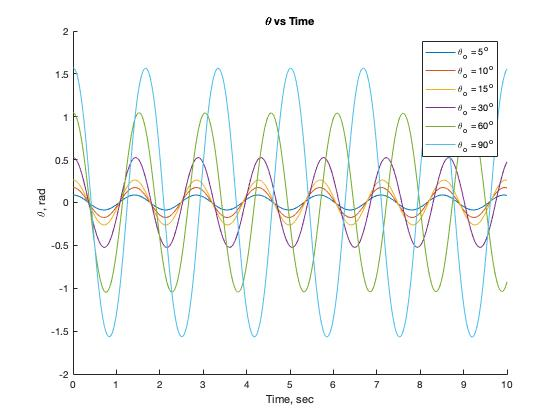
\includegraphics [width=5in,center]{Pendulum_01.jpg}

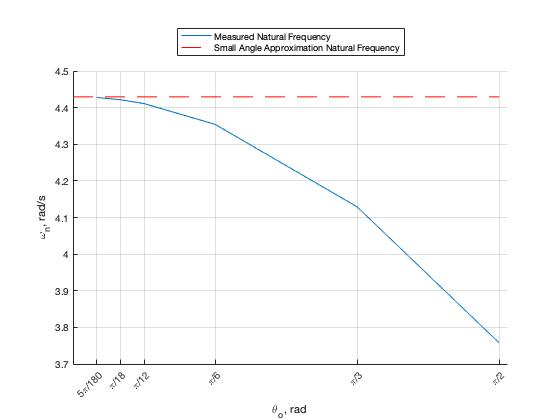
\includegraphics [width=5in,center]{Pendulum_02.jpg}
